% Compile: xelatex formulation.tex  (run from tex/, twice)
\documentclass[11pt,a4paper]{article}
\usepackage{kotex}
\setmainhangulfont{AppleMyungjo}[AutoFakeBold=2.5,AutoFakeSlant=0.15]
\setsanshangulfont{Apple SD Gothic Neo}
\usepackage[margin=24mm]{geometry}
\usepackage{amsmath,amssymb,amsthm}
\usepackage{booktabs}
\usepackage{graphicx}
\usepackage{float}
\usepackage{enumitem}
\usepackage{tikz}
\usepackage[hidelinks]{hyperref}
\setlist{itemsep=2pt,topsep=4pt}

\newtheorem{lemma}{Lemma}
\newtheorem{proposition}{Proposition}
\renewcommand{\Re}{\operatorname{Re}}
\renewcommand{\Im}{\operatorname{Im}}
\newcommand{\Fb}{\bar F}
\newcommand{\Rot}{\operatorname{Rot}}

\title{CKKS 기반 동적 제어기:\\ TAC--ARX 지연 입력창 구조, bootstrapping, 허수부 문제}
\author{}
\date{2026-09-29}

\begin{document}
\maketitle

\begin{abstract}
\begin{itemize}
\item 불안정한 내부 행렬 $F$를 가질 수 있는 선형 동적 제어기를 CKKS로 무한 시간 운용하는 구조를 정리함.
\item TAC에서 deadbeat $R$을 쓰면 제어기 상태가 최근 $n$개 입출력으로 결정되는 ARX 표현을 얻음.
      여기에 순방향 전파를 결합해, bootstrapping된 과거 입력창과 fresh 출력만으로 매 step $u(t)$를 계산하는 지연 입력창 식을 유도함.
\item 입력창을 $K$ step 재사용해 bootstrapping에 $d$ period의 여유를 줌.
      단, 리셋 오차가 누적되지 않으려면 $d\le K-n+1$이어야 함.
\item Re-encryption을 bootstrapping으로 대체하면 CKKS 허수부가 plant를 거치지 않고 $F$로 개루프 전파되어 발산함.
      Bootstrapping 직후 conjugation으로 허수부를 제거하면 해결됨.
\item CT-CT 구현에서 $u$는 4-slot sparse를 유지하고, $y$와 입력창을 패킹함.
      $u$ 계산은 $K$에 대해 로그로만 늘고, bootstrapping은 창당 1회임.
\item 128-bit ($N=65536$), $K=64$, $d=61$에서 약 6\,s의 bootstrapping을 흡수함.
      Sampling period 약 0.3\,s에서 $u$ 오차가 $1.1\times10^{-7}$ 이하로 유계임.
\end{itemize}
\end{abstract}

\tableofcontents

%==========================================================================
\section{배경과 작업 경과}

동료 저장소(단계 01--04)에서 출발함. 진행 순서는 다음과 같음.

\begin{enumerate}
\item \textbf{기존 구현 재현.}
  \begin{itemize}
  \item 01 평문 TAC, 02 평문 u/y reconstruction, 03 PT-CT, 04 CT-CT를 OpenFHE v1.5.1로 재현함.
  \item 40 step 실험에서는 모든 profile의 오차가 $10^{-8}$ 이하였음.
  \end{itemize}
\item \textbf{발산 현상 확인.}
  \begin{itemize}
  \item 동료가 보고한 ``$u$ 오차가 선형 증가''하는 현상을 500 step에서 확인함.
  \item 실제로는 지수 증가였음 (로그 축에서 직선). 증가율은 block당 약 1.197배였음.
  \item 03 unstable profile은 360 step대에서 복호화가 실패함.
  \end{itemize}
\item \textbf{원인 규명: 허수부.}
  \begin{itemize}
  \item Bootstrapping은 CKKS slot의 허수부를 보존함. Plant는 실수부만 받음.
  \item 따라서 허수부가 폐루프를 거치지 않고 $F$로 개루프 전파됨 (\S\ref{sec:imag}).
  \item 허수부 오차 추정치의 증가율이 $\rho(F)^4$과 일치함을 확인함.
  \end{itemize}
\item \textbf{해결.}
  \begin{itemize}
  \item 03에 \texttt{--clear-imag}를 추가함 (conjugation으로 허수부 제거).
  \item Unstable profile에서도 오차가 $10^{-8}$에서 유지됨.
  \end{itemize}
\item \textbf{구조 재정립: TAC와 ARX.}
  \begin{itemize}
  \item 기존 u/y reconstruction이 deadbeat TAC의 ARX 형태와 같음을 확인함.
  \item ``bootstrapping된 입력창을 $K$ step 재사용해 시간을 버는'' 구조를 지연 입력창 식으로 유도함 (\S\ref{sec:window}).
  \end{itemize}
\item \textbf{CT-CT 구현 (05).}
  \begin{itemize}
  \item 초기화, 실시간 스케줄 모델, 허수부 제거를 포함함.
  \item 스칼라 방식은 $K$에 비례해 곱셈이 늘어 $u$ 계산이 병목이 됨.
  \end{itemize}
\item \textbf{패킹 최적화.}
  \begin{itemize}
  \item $u$는 4-slot sparse를 유지하고 $y$를 zero-padded rotation으로 패킹함. $u$ 계산이 $K$에 대해 로그로만 늘어남.
  \item 입력창을 bootstrapping 전에 패킹해 bootstrapping을 창당 1회로 줄임.
  \end{itemize}
\item \textbf{128-bit 평가.}
  \begin{itemize}
  \item 128-bit ($N=65536$)에서 bootstrapping이 약 5--6\,s임을 측정함.
  \item 메모리 때문에 입력을 필요한 레벨로만 암호화함 (compact inputs).
  \item $K=16,32,64$ ($d=K$)를 비교해 여유가 넉넉한 $K=64$를 택함.
  \end{itemize}
\item \textbf{리셋 점프 누적 발견.}
  \begin{itemize}
  \item $K=d=64$를 1000 step 돌리자 오차가 block당 6.8배로 발산함.
  \item 평문 시뮬레이션에서도 같은 증가율이 나옴. CKKS가 아니라 지연 입력창 구조의 문제임.
  \item 원인은 입력창이 이전 블록의 리셋 시점을 포함하는 것임 (\S\ref{sec:dstab}).
  \item 조건 $d\le K-n+1$이면 해결됨. 최종 설정 $K=64$, $d=61$에서 640 step 유계를 확인함 (\S\ref{sec:128}).
  \end{itemize}
\end{enumerate}

%==========================================================================
\section{문제 설정}

\paragraph{Plant와 제어기.}
\begin{align}
x_p(t+1)&=Ax_p(t)+Bu(t), & y(t)&=Cx_p(t), \label{eq:plant}\\
x(t+1)&=Fx(t)+Gy(t), & u(t)&=Hx(t). \label{eq:ctrl}
\end{align}
\begin{itemize}
\item SISO이고, 제어기 차수는 $n$임 (본 실험 $n=4$).
\item $(F,H)$는 observable임.
\item 폐루프 행렬은 다음과 같고 안정함.
\end{itemize}
\begin{equation}
A_{cl}=\begin{bmatrix}A&BH\\GC&F\end{bmatrix},\qquad \rho(A_{cl})<1 .
\end{equation}
\begin{itemize}
\item $F$ 자체는 불안정할 수 있음.
\end{itemize}
\begin{equation}
\rho(F)>1 .
\end{equation}

\paragraph{Profile.}
\begin{itemize}
\item \texttt{stable}: $\rho(F)=0.6$, $\rho(A_{cl})=0.689$.
\item \texttt{unstable\_low}: $\rho(F)=1.046$, $\rho(A_{cl})=0.785$.
\item \texttt{unstable\_high}: \texttt{unstable\_low}의 비정규 좌표변환. 이상적 입출력은 동일함.
\end{itemize}

\paragraph{암호화 환경.}
\begin{itemize}
\item 센서는 매 step $y(t)$를 새로 암호화함. 따라서 $y$는 레벨이 가득 찬 fresh 암호문임.
\item 센서는 과거 $y$를 저장하지 않음.
\item 서버(제어기)는 암호문으로 $u(t)$를 계산함.
\item 액추에이터는 $u$를 복호화해 실수부를 plant에 인가함.
\item $u$ 암호문을 다시 쓰려면 레벨 회복이 필요함. 이를 bootstrapping으로 함.
\item Bootstrapping 시간 $T_{\mathrm{bt}}$는 sampling period $T_s$보다 길 수 있음.
\item 최종 목표는 계수까지 암호화하는 CT-CT임.
\end{itemize}

\paragraph{목표.}
\begin{enumerate}
\item[(G1)] 상태 $x$를 암호문으로 유지하지 않음. 과거 $u,y$의 선형결합으로 $u(t)$를 계산함 (ARX).
\item[(G2)] 사용하는 과거 $u$는 bootstrapping이 끝난 것이어야 함.
\item[(G3)] 같은 입력창을 $K$ step 재사용해 bootstrapping 시간을 확보함.
\item[(G4)] 결과가 원래 제어기 \eqref{eq:ctrl}와 정확히 같아야 함. 그래야 폐루프 안정성이 유지됨.
\end{enumerate}

%==========================================================================
\section{제어기 표현: TAC와 ARX}

\subsection{Re-encryption 기반 변환 (TAC)}
\begin{itemize}
\item Kim~\cite{kim}의 변환: 임의의 $R\in\mathbb R^n$에 대해 다음과 같이 씀.
\end{itemize}
\begin{equation}
x(t+1)=\Fb x(t)+Gy(t)+Ru(t),\qquad \Fb:=F-RH .
\label{eq:tac}
\end{equation}
\begin{itemize}
\item $u(t)=Hx(t)$가 되먹임되면 다음이 성립해 \eqref{eq:ctrl}과 같아짐.
\end{itemize}
\begin{equation}
\Fb x+Ru=Fx .
\end{equation}
\begin{itemize}
\item \textbf{핵심 조건:} plant에 인가된 것과 \emph{같은} $u(t)$가 제어기에 되먹임되어야 함~\cite[Sec.~I-A]{kim}.
\item 이 조건이 성립하면 암호화 오차는 plant와 제어기가 공유하는 외란이 됨.
\item 오차 동역학은 $A_{cl}$을 따름.
\end{itemize}

\subsection{Deadbeat 선택과 ARX 표현}
\begin{lemma}[Deadbeat $R$]
$(F,H)$가 observable이면 아래 $R$에 대해 $\Fb^{\,n}=0$임.
\begin{equation}
R=F^n\mathcal O^{-1}e_n,\qquad \mathcal O=\begin{bmatrix}H\\HF\\\vdots\\HF^{n-1}\end{bmatrix}.
\label{eq:R}
\end{equation}
\end{lemma}
\begin{proof}
관측기 이득의 Ackermann 공식에서 목표 특성다항식을 $z^n$으로 둔 경우임.
\end{proof}

\begin{lemma}[ARX 표현]
\eqref{eq:R}의 $R$에 대해 모든 $\tau$에서 다음이 성립함.
\begin{equation}
x(\tau+1)=\sum_{j=0}^{n-1}\Fb^{\,j}\bigl(G\,y(\tau-j)+R\,u(\tau-j)\bigr).
\label{eq:arx-state}
\end{equation}
\end{lemma}
\begin{proof}
\eqref{eq:tac}를 $n$ step 전개하면 $\Fb^{\,n}x(\tau-n+1)$ 항이 남음. 이 항은 0임.
\end{proof}

\paragraph{기존 u/y reconstruction과의 관계.}
\begin{itemize}
\item 기존 구현(02--04)은 다음으로 상태를 재구성함 ($K=n=4$).
\end{itemize}
\begin{equation}
x(t+K)=M_uU+M_yY,\qquad M_u=F^4\mathcal O^{-1}.
\end{equation}
\begin{itemize}
\item 이것은 \eqref{eq:arx-state}와 정확히 같음. 수치 확인 결과는 다음과 같음.
\end{itemize}
\begin{equation}
\bigl\|M_u-[\Fb^3R,\ \Fb^2R,\ \Fb R,\ R]\bigr\|\le3\times10^{-14}.
\end{equation}
\begin{itemize}
\item $R$은 $M_u$의 마지막 열임.
\item 즉 u/y reconstruction은 deadbeat TAC의 ARX 형태임.
\end{itemize}

%==========================================================================
\section{지연 입력창 ARX 제어 입력}\label{sec:window}

\subsection{유도}
\begin{itemize}
\item 시간을 길이 $K$의 블록으로 나눔. 블록 $k$는 다음 구간임.
\end{itemize}
\begin{equation}
t=kK,\ \dots,\ kK+K-1 .
\end{equation}
\begin{itemize}
\item 블록 $k$는 다음 입력창을 씀. $d$는 입력창의 지연임.
\end{itemize}
\begin{equation}
W_k=\bigl[u(\tau_k-n+1),\dots,u(\tau_k)\bigr],\qquad \tau_k=kK-d,\quad d\ge1 .
\end{equation}
\begin{itemize}
\item $\tau_k+1$ 이후에는 $u$를 쓰지 않는 원래 형태 \eqref{eq:ctrl}로 전파함.
\end{itemize}
\begin{equation}
x(t)=F^{\,t-\tau_k-1}x(\tau_k+1)+\sum_{s=\tau_k+1}^{t-1}F^{\,t-1-s}Gy(s).
\label{eq:forward}
\end{equation}

\begin{proposition}[지연 입력창 ARX]
$t=kK+i$에 대해 다음을 정의함.
\begin{equation}
m=t-\tau_k-1=d+i-1 .
\end{equation}
그러면 다음이 성립함.
\begin{equation}
\boxed{\;u(t)=\sum_{j=0}^{n-1}\alpha_{m,j}\,u(\tau_k-j)+\sum_{j=0}^{n-1}\beta_{m,j}\,y(\tau_k-j)+\sum_{l=0}^{m-1}\gamma_l\,y(t-1-l)\;}
\label{eq:main}
\end{equation}
\begin{equation}
\alpha_{m,j}=HF^m\Fb^{\,j}R,\qquad\beta_{m,j}=HF^m\Fb^{\,j}G,\qquad\gamma_l=HF^lG .
\label{eq:coef}
\end{equation}
입력창의 $u$가 인가된 $u$와 같으면 \eqref{eq:main}은 $u(t)=Hx(t)$와 정확히 같음.
\end{proposition}
\begin{proof}
$u(t)=Hx(t)$에 \eqref{eq:forward}와 \eqref{eq:arx-state}를 대입함.
\end{proof}

\subsection{성질}
\begin{itemize}
\item \textbf{상태변수 없음.} $u(t)$는 입력창 $n$개와 출력 $n+m$개의 선형결합임.
\item \textbf{곱셈 깊이 1.} 모든 계수는 오프라인 계산임. $u(t)$ 하나당 계수$\times$신호 곱셈 한 단이면 됨.
\item \textbf{Realization 불변.} 좌표변환에 대해 다음이 성립함.
\end{itemize}
\begin{equation}
(F,G,H)\to(TFT^{-1},TG,HT^{-1})\ \Rightarrow\ R\to TR,\quad \Fb\to T\Fb T^{-1}.
\end{equation}
\begin{itemize}
\item[] 따라서 \eqref{eq:coef}의 계수가 모두 불변임. \texttt{unstable\_low}와 \texttt{unstable\_high}의 계수가 같음.
\item \textbf{계수 증가.} 계수 크기는 다음과 같이 커짐. 입력창 오차가 이만큼 증폭될 수 있음.
\end{itemize}
\begin{equation}
|\alpha_{m,j}|,\ |\beta_{m,j}|\sim\rho(F)^{m},\qquad m\le d+K-2 .
\end{equation}
\begin{itemize}
\item \textbf{기존 구현과의 관계.} $d=1$, $K=n$인 경우가 기존 구현임.
\end{itemize}

\subsection{블록 리셋 점프와 지연 $d$의 안정 조건}\label{sec:dstab}

\paragraph{이 구조에서 ``블록''과 ``리셋''이란.}
\begin{itemize}
\item 원래 제어기 \eqref{eq:ctrl}은 상태 $x(t)$ 하나를 계속 이어서 갱신함.
\item 우리 구조는 상태를 암호문으로 들고 다니지 않음. 대신 블록마다 제어기 상태를 \emph{새로 만듦}.
  \begin{itemize}
  \item 블록 $k$가 시작되면, 입력창(bootstrapping된 과거 $u$ 4개)과 그 시점의 $y$로 시작 상태 $\tilde x_k$를 계산함 (ARX 복원).
  \item 블록 $k$ 동안은 이 시작 상태에서 $x^+=Fx+Gy$로 앞으로 굴린 값을 써서 $u(t)=Hx(t)$를 냄.
  \item 식 \eqref{eq:main}은 이 과정을 계수 하나로 합친 것임.
  \end{itemize}
\item 즉 블록마다 ``입력창에서 출발하는 새 제어기 궤적''을 씀.
\item 블록이 바뀔 때 이전 블록의 궤적을 버리고 새 궤적으로 갈아타는 것을 \emph{리셋}이라 부름.
\end{itemize}

\paragraph{블록 점프란.}
\begin{itemize}
\item 블록 경계 시각 $kK$에서 두 값을 비교할 수 있음.
  \begin{itemize}
  \item 이전 블록 궤적을 계속 굴렸다면 가졌을 상태: $\hat x_{k-1}(kK)$.
  \item 새 블록이 입력창에서 계산한 상태: $\hat x_k(kK)$.
  \end{itemize}
\item 두 값의 차이가 \emph{블록 점프}임.
\end{itemize}
\begin{equation}
J_k=\hat x_k(kK)-\hat x_{k-1}(kK).
\end{equation}
\begin{itemize}
\item 제어기 상태가 블록 경계에서 순간적으로 $J_k$만큼 튀는 것과 같음.
\item 그림 \ref{fig:final-d}의 톱니 모양에서 블록 시작마다 오차가 튀어 오르는 지점이 점프임.
\end{itemize}

\paragraph{점프는 왜 생기나.}
\begin{itemize}
\item 오차가 전혀 없으면 점프는 0임.
  \begin{itemize}
  \item ARX 항등식 \eqref{eq:arx-state} 때문에, 입력창에서 복원한 상태가 이전 궤적의 상태와 정확히 같음.
  \end{itemize}
\item CKKS 오차가 있으면 두 값이 어긋남.
  \begin{itemize}
  \item 이전 블록 궤적은 ``$u=Hx$가 정확히 인가됐다''고 보고 굴린 값임.
  \item 실제로 인가된 $u$에는 계산 오차 $n$이 있고, 입력창 사본에는 bootstrapping 오차 $\delta$도 있음.
  \item 새 블록은 이 오차가 실린 $u$로 상태를 복원함.
  \item 그래서 복원값에 창의 오차가 반영되고, 이전 궤적과 차이가 남.
  \end{itemize}
\item 즉 점프는 ``입력창에 실린 CKKS 오차가 리셋 때 제어기 상태로 옮겨진 흔적''임.
\item 이 차이는 창 시점부터 블록 시작까지 $F^{d-1}$로 전파됨. 그래서 $F$가 불안정하고 $d$가 크면 점프가 커짐.
      이것이 계수 증폭 $\rho(F)^{2K-2}$의 실체임.
\end{itemize}

\paragraph{점프가 괜찮은 경우와 문제가 되는 경우.}
\begin{itemize}
\item \textbf{괜찮은 경우: 점프가 매번 새로 생기는 작은 충격일 때.}
  \begin{itemize}
  \item 각 점프가 그 블록 입력창의 오차에만 의존하면, 점프 크기는 유계임.
  \item 폐루프 $A_{cl}$이 안정하므로 이런 충격은 블록 안에서 감쇠함 (톱니 높이가 일정).
  \end{itemize}
\item \textbf{문제가 되는 경우: 점프가 다음 점프를 낳을 때.}
  \begin{itemize}
  \item 입력창이 이전 블록의 경계(리셋 시점)를 포함하면, 창의 샘플 일부는 리셋 전 궤적, 일부는 리셋 후 궤적에서 나온 것임.
  \item ARX 복원은 창이 한 궤적에서 왔다고 가정하므로, 이전 점프를 궤적의 일부로 잘못 해석함.
  \item 그 잘못 해석된 성분이 새 시작 상태에 섞여 다음 블록까지 $F^{d-1}$로 전파되고, 다음 점프가 됨.
  \item 이 재귀는 제어기 내부에서만 돔. $y$는 양쪽에 똑같이 들어가 상쇄되므로 plant가 바로잡지 못함.
  \item 배율이 1보다 크면 폐루프가 안정해도 점프가 블록마다 커져 발산함.
  \end{itemize}
\item 어느 경우인지는 입력창 위치, 즉 지연 $d$가 정함 (그림 \ref{fig:jump-timeline}).
\end{itemize}

\paragraph{비유: 이어달리기.}
\begin{itemize}
\item 각 블록의 제어기는 새로 출발하는 주자임.
\item 새 주자는 이전 주자의 최근 발자국 4개(입력창)를 보고 자기 출발 위치를 정함.
\item 발자국이 조금 흐리면(CKKS 오차) 출발 위치가 조금 어긋남. 이것이 점프임.
\item 발자국 4개가 모두 이전 주자 한 명의 것이면, 어긋남은 매번 새로 생기는 작은 오차일 뿐임.
\item 그런데 발자국에 그 전 바톤 터치 지점(이전 주자가 출발하며 어긋났던 곳)이 섞이면, 새 주자는 그 어긋남까지 이어받음.
      이게 매번 반복되면서 커지는 것이 발산임.
\end{itemize}

\paragraph{발견 경위.}
\begin{itemize}
\item Proposition 1의 등식은 입력창 $u$가 인가된 $u$와 \emph{정확히} 같을 때만 성립함.
\item 처음에는 이것만으로 충분하다고 봤음. 폐루프가 안정하니 CKKS 오차는 유계 외란으로 흡수될 것이라고 봤음.
\item 그러나 128-bit, $K=d=64$에서 1000 step을 돌리자 오차가 block당 6.8배로 발산함.
\item 같은 설정을 암호화 없이 평문 + $10^{-12}$ 노이즈로 돌려도 증가율이 6.83으로 같았음.
\item 즉 CKKS 문제가 아니라 \emph{구현 구조}(블록마다 상태를 다시 만드는 방식)의 문제였음.
\end{itemize}

\paragraph{구현이 실제로 하는 일.}
\begin{itemize}
\item 식 \eqref{eq:main}은 블록 $k$마다 다음 \emph{가상 상태 궤적}을 쓰는 것과 같음.
\end{itemize}
\begin{equation}
\hat x_k(\tau_k+1)=\tilde x_k,\qquad \hat x_k(t+1)=F\hat x_k(t)+Gy(t),\qquad u(t)=H\hat x_k(t)+n(t)\quad(t\in\text{블록 }k).
\end{equation}
\begin{itemize}
\item 여기서 $n(t)$는 CKKS 출력 오차, $\tilde x_k$는 입력창으로 계산한 시작 상태임 ($\delta$: bootstrapping 오차).
\end{itemize}
\begin{equation}
\tilde x_k=\sum_{j=0}^{n-1}\Fb^{\,j}\bigl(Gy(\tau_k-j)+Ru_{\mathrm{bt}}(\tau_k-j)\bigr),\qquad u_{\mathrm{bt}}=u+\delta .
\end{equation}
\begin{itemize}
\item 블록이 바뀌면 사용하는 궤적이 $\hat x_{k-1}$에서 $\hat x_k$로 바뀜. 이를 \emph{리셋}이라 부름.
\item 노이즈가 없으면 두 궤적은 같음. 노이즈가 있으면 블록 경계에서 불연속(점프)이 생김.
\end{itemize}
\begin{equation}
J_k:=\hat x_k(kK)-\hat x_{k-1}(kK).
\end{equation}
\begin{itemize}
\item 두 궤적은 같은 $y$로 같은 $F$ 재귀를 따르므로 다음이 성립함.
\end{itemize}
\begin{equation}
J_k=F^{\,d-1}\bigl(\tilde x_k-\hat x_{k-1}(\tau_k+1)\bigr).
\label{eq:jump-def}
\end{equation}

\paragraph{직관: 입력창은 ``끊김 없는 한 궤적''을 가정함.}
\begin{itemize}
\item ARX 복원 \eqref{eq:arx-state}는 창의 $n$개 샘플이 \eqref{eq:ctrl}의 한 궤적에서 나왔다고 가정함.
\item 창이 한 블록 안에 있으면 이 가정이 맞음. 복원 오차는 그 창의 노이즈뿐임.
\item 창이 블록 경계에 걸치면, 창 안에 이전 리셋 점프 $J_{k-1}$이 들어 있음.
\item 복원은 이 점프를 궤적의 일부로 \emph{잘못 해석}함. 그 결과 $\tilde x_k$에 점프를 걸러낸 성분 $\Fb^{\,p}J_{k-1}$이 섞임.
\item 이 성분은 다음 블록 시작까지 $F^{d-1}$로 전파되어 다음 점프 $J_k$가 됨.
\item 즉 점프가 점프를 낳는 재귀가 생김. $\rho(F)>1$이고 $d$가 크면 증폭됨.
\end{itemize}

\begin{figure}[H]
\centering
\begin{tikzpicture}[x=0.62cm,y=1cm,font=\small]
  \draw[->] (3.3,0) -- (22.8,0) node[right] {$t$};
  \foreach \x in {4,...,22} \fill (\x,0) circle (1.8pt);
  \foreach \x/\lab in {8/{(k-1)K},16/{kK}} {
    \draw[dashed,red!70!black] (\x-0.5,-2.0) -- (\x-0.5,2.0);
    \node[red!70!black,below] at (\x-0.5,-2.0) {$\lab$};
  }
  \node[red!70!black] at (19.2,1.6) {블록 경계 = 리셋};
  \node at (5.5,0.35) {블록 $k-2$};
  \node at (11.5,0.35) {블록 $k-1$};
  \node at (19.5,0.35) {블록 $k$};
  % d = K: window samples 5..8 straddle the reset at (k-1)K
  \draw[rounded corners,thick,orange!85!black,fill=orange!15] (4.6,1.0) rectangle (8.4,1.5);
  \node[orange!85!black,left] at (4.5,1.25) {$d=K$};
  \node[orange!85!black,above,align=center] at (5.2,1.5) {이전 리셋 포함\\$\Rightarrow$ 점프 전달};
  % d = K-n+1: window samples 8..11 inside block k-1
  \draw[rounded corners,thick,blue!70!black,fill=blue!12] (7.6,-1.0) rectangle (11.4,-1.5);
  \node[blue!70!black,left] at (7.3,-1.25) {$d=K-n+1$};
  \node[blue!70!black,below,align=center] at (11.8,-1.5) {한 블록 안\\$\Rightarrow$ 점프는 매번 독립};
\end{tikzpicture}
\caption{블록 $k$의 입력창 위치 ($K=8$, $n=4$ 예시). $d=K$이면 창이 블록 $k-1$의 리셋 시점을 포함함. $d=K-n+1$이면 창이 블록 $k-1$ 안에만 있음.}
\label{fig:jump-timeline}
\end{figure}

\paragraph{유도.}
\begin{lemma}[점프가 있는 ARX 항등식]
창 구간 $[\tau-n+1,\tau]$에서 실제로 쓰인 상태를 $\hat x_{\mathrm{act}}$라 함.
$\hat x_{\mathrm{act}}$는 $F$ 재귀를 따르되, 어떤 시각 $s_0$로 넘어갈 때만 $J$만큼 점프한다고 함.
\begin{equation}
\hat x_{\mathrm{act}}(s+1)=F\hat x_{\mathrm{act}}(s)+Gy(s)+J\cdot\mathbf 1[s+1=s_0],\qquad u(s)=H\hat x_{\mathrm{act}}(s)+n(s).
\end{equation}
그러면 다음이 성립함.
\begin{equation}
\sum_{j=0}^{n-1}\Fb^{\,j}\bigl(Gy(\tau-j)+Ru_{\mathrm{bt}}(\tau-j)\bigr)
=\hat x_{\mathrm{act}}(\tau+1)+\sum_{j=0}^{n-1}\Fb^{\,j}R\,(n+\delta)(\tau-j)-\Fb^{\,\tau+1-s_0}J .
\end{equation}
단, $\tau+1-s_0\ge n$이거나 $s_0$가 창 밖이면 마지막 항은 0임.
\end{lemma}
\begin{proof}
\begin{itemize}
\item $x_T(s+1)=\Fb x_T(s)+Gy(s)+Ru_{\mathrm{bt}}(s)$로 두고 $e:=x_T-\hat x_{\mathrm{act}}$라 함.
\item $F=\Fb+RH$이므로 다음이 성립함.
\end{itemize}
\begin{equation}
e(s+1)=\Fb e(s)+R(n+\delta)(s)-J\cdot\mathbf 1[s+1=s_0].
\end{equation}
\begin{itemize}
\item $n$ step 전개하면 초기값 항은 $\Fb^{\,n}=0$으로 사라짐. 남는 항이 위 식임.
\end{itemize}
\end{proof}

\begin{proposition}[점프 재귀]
블록 $k$의 창 $[\tau_k-n+1,\tau_k]$에 대해 다음을 정의함.
\begin{equation}
p:=\tau_k+1-(k-1)K=K-d+1 .
\end{equation}
\begin{itemize}
\item $p\ge n$ (즉 $d\le K-n+1$): 창이 블록 $k-1$ 안에 있음. 점프는 현재 창의 노이즈에만 의존함.
\end{itemize}
\begin{equation}
J_k=F^{\,d-1}\sum_{j=0}^{n-1}\Fb^{\,j}R\,(n+\delta)(\tau_k-j)=:w_k .
\end{equation}
\begin{itemize}
\item $1\le p\le n-1$ (즉 $K-n+1<d\le K$): 창이 블록 $k-1$의 리셋을 포함함. 이전 점프가 전달됨.
\end{itemize}
\begin{equation}
J_k=-F^{\,d-1}\Fb^{\,K-d+1}J_{k-1}+w_k .
\label{eq:jump-rec}
\end{equation}
\end{proposition}
\begin{proof}
Lemma를 $s_0=(k-1)K$, $J=J_{k-1}$로 적용하고, $\hat x_{\mathrm{act}}(\tau_k+1)=\hat x_{k-1}(\tau_k+1)$을 이용해 \eqref{eq:jump-def}에 대입함.
\end{proof}

\paragraph{안정 조건.}
\begin{itemize}
\item 점프 수열 $\{J_k\}$가 유계일 필요충분조건은 다음과 같음.
\end{itemize}
\begin{equation}
\rho\bigl(M_d\bigr)<1,\qquad M_d:=F^{\,d-1}\Fb^{\,K-d+1}.
\label{eq:dstab}
\end{equation}
\begin{itemize}
\item $d\le K-n+1$이면 $\Fb^{\,K-d+1}=0$이라 $M_d=0$임. 재귀 자체가 없어짐 (충분조건).
\item $d=K$이면 $M_K=F^{K-1}\Fb$임. $\rho(F)>1$이면 대략 $\rho(F)^{K}$로 커짐.
\item 기존 구현($d=1$, $K=n=4$)은 $p=4=n$이라 조건을 만족함. 그래서 발산이 없었음.
\end{itemize}

\paragraph{폐루프에 미치는 영향.}
\begin{itemize}
\item 구현된 폐루프 $[x_p;\hat x_{\mathrm{act}}]$는 블록 안에서 $A_{cl}$을 그대로 따름.
\item 여기에 두 종류의 외란이 더해짐.
  \begin{itemize}
  \item 매 step 입력 외란 $B\,n(t)$.
  \item 블록 경계마다 제어기 상태 점프 $J_k$.
  \end{itemize}
\end{itemize}
\begin{equation}
\begin{bmatrix}x_p\\ \hat x_{\mathrm{act}}\end{bmatrix}(t+1)=A_{cl}\begin{bmatrix}x_p\\ \hat x_{\mathrm{act}}\end{bmatrix}(t)+\begin{bmatrix}B\\0\end{bmatrix}n(t)+\begin{bmatrix}0\\ J_k\end{bmatrix}\mathbf 1[t+1=kK].
\end{equation}
\begin{itemize}
\item $\rho(A_{cl})<1$이므로 $J_k$가 유계이면 전체 오차도 유계임.
\item 그러나 $A_{cl}$은 점프 수열 자체를 줄여주지 못함.
  \begin{itemize}
  \item 식 \eqref{eq:jump-rec}에서 $y$ 항은 $\tilde x_k$와 $\hat x_{k-1}$에 똑같이 들어가 상쇄됨.
  \item 즉 점프 재귀는 plant를 거치지 않는 \emph{제어기 내부의 개루프 재귀}임.
  \end{itemize}
\item 그래서 폐루프가 안정해도 $\rho(M_d)>1$이면 발산함.
\item 그림 \ref{fig:final-d}의 톱니 모양이 이것임. 블록 시작마다 점프가 들어오고 블록 안에서 $A_{cl}$로 감쇠함. $d=K$이면 톱니 높이가 매 블록 6.8배씩 커짐.
\end{itemize}

\paragraph{허수부 문제와의 비교.}
\begin{itemize}
\item 두 문제 모두 ``폐루프가 안정한데도 발산''함. 원인은 plant가 보지 못하는 경로로 오차가 도는 것임.
\item 허수부: plant가 허수부를 관측하지 못함. $F$로 매 step 개루프 전파됨.
\item 리셋 점프: 점프 재귀가 제어기 내부에서만 돔. $M_d$로 매 블록 개루프 전파됨.
\item Kim의 조건 ``인가된 $u$ = 되먹임되는 $u$''는 제어기가 매 step 하나의 재귀로 돈다고 가정함.
      블록마다 상태를 다시 만드는 구현에서는 이것만으로 부족하고, 리셋 구조의 안정성을 따로 확인해야 함.
\end{itemize}

\paragraph{수치 확인.}
\begin{table}[H]
\centering
\begin{tabular}{lrrrr}
\toprule
\texttt{unstable\_low}, $d=K$ & $K=16$ & 32 & 64 & 128 \\
\midrule
예측 $\rho(F^{K-1}\Fb)$ & 0.789 & 1.62 & 6.83 & 122 \\
평문 시뮬레이션 증가율 (block당) & 유계 & 1.61 & 6.83 & 121.8 \\
128-bit CKKS 증가율 (block당) & -- & -- & 약 6.8 & -- \\
\midrule
$d=K-3$에서 마지막 block 오차 & $4\times10^{-12}$ & $3\times10^{-12}$ & $6\times10^{-12}$ & $3\times10^{-10}$ \\
\bottomrule
\end{tabular}
\caption{$d=K$일 때 예측과 측정. 평문 시뮬레이션은 $u$와 bootstrapping 사본에 $10^{-12}$ 노이즈를 넣음. \texttt{unstable\_high}도 같은 값 (realization 불변). \texttt{stable}은 모든 경우 유계.}
\label{tab:dstab}
\end{table}

\begin{table}[H]
\centering
\begin{tabular}{lrrrr}
\toprule
$K=64$ & $d=64$ & $d=63$ & $d=62$ & $d=61$ \\
\midrule
$p=K-d+1$ & 1 & 2 & 3 & 4 \\
$\rho(M_d)$ & 6.83 & 0.767 & 0.422 & 0 \\
\bottomrule
\end{tabular}
\caption{$d$를 한 칸씩 줄일 때의 점프 배율 (\texttt{unstable\_low}). $\|\Fb\|=1.75$, $\|\Fb^2\|=1.41$, $\|\Fb^3\|=0.31$로 $p$가 클수록 빠르게 작아짐.}
\label{tab:dscan}
\end{table}
\begin{itemize}
\item 예측이 평문 시뮬레이션과 CKKS 결과에 모두 정확히 맞음.
\item $K=64$에서는 $d=63$만 되어도 $\rho<1$임. 하지만 0.77이면 감쇠가 느림.
\item $d\le K-n+1$이면 재귀가 완전히 사라져 가장 안전함.
\end{itemize}

\paragraph{설계 지침.}
\begin{itemize}
\item 기본값으로 $d=K-n+1$을 씀. 05 구현도 $d$를 지정하지 않으면 이 값을 쓰고, 조건을 넘으면 경고를 출력함.
\item 포기하는 bootstrapping 여유는 $n-1$ period뿐임 ($K=64$에서 64$\to$61).
\item $d\le K-n+1$일 때 남는 점프 크기는 다음과 같음. 이것이 계수 증폭 $\rho(F)^{2K-2}$의 실체임.
\end{itemize}
\begin{equation}
\|J_k\|\lesssim\|F^{\,d-1}\|\,\max_j\|\Fb^{\,j}R\|\,\max|n+\delta| .
\end{equation}
\begin{itemize}
\item[] ($K=64$, $d=61$에서 $\|F^{60}\Fb^{\,j}R\|$는 최대 약 8.4임.)
\item 다른 대안도 생각할 수 있음. 다만 모두 구현이 복잡해서 채택하지 않음.
  \begin{itemize}
  \item 이전 점프를 추정해 보정하는 방법. 점프가 암호문이라 추가 연산이 필요함.
  \item 창 길이를 $n$보다 늘리는 방법. 창이 경계에 걸치면 같은 문제가 남음.
  \end{itemize}
\end{itemize}

\paragraph{시간 확보와의 관계.}
\begin{itemize}
\item $d=K-n+1$이면 bootstrapping 여유는 $K-n+1$ period임.
\item 입력창 패킹 시 처리량은 여전히 step당 $1/K$회임.
\end{itemize}

\subsection{초기화}
\begin{itemize}
\item 첫 입력창이 채워지는 시점은 다음과 같음.
\end{itemize}
\begin{equation}
t^\star=k^\star K,\qquad k^\star=\bigl\lceil(n-1+d)/K\bigr\rceil .
\end{equation}
\begin{itemize}
\item $t<t^\star$에서는 초기 상태를 씀.
\end{itemize}
\begin{equation}
u(t)=HF^t x(0)+\sum_{l=0}^{t-1}\gamma_l\,y(t-1-l).
\label{eq:init}
\end{equation}
\begin{itemize}
\item $x(0)$은 설정 단계에서 한 번 암호화해 전달함.
\item 이 식도 곱셈 깊이 1임.
\end{itemize}

\subsection{Bootstrapping 일정과 실시간 조건}
\begin{itemize}
\item 입력창에 들어가는 $u$만 bootstrapping함.
\item 연속한 입력창은 $\min(n,K)$개 원소만 다름. 따라서:
\end{itemize}
\begin{equation}
\text{step당 bootstrapping 횟수}=\frac{\min(n,K)}{K}.
\end{equation}
\begin{itemize}
\item $W_{k+1}$의 마지막 원소 $u((k+1)K-d)$는 시각 $(k+1)K$에 처음 쓰임. 즉 여유는 $d$ period임.
\item $T_u$를 step당 서버 계산 시간이라 하면 실시간 조건은 다음과 같음.
\end{itemize}
\begin{equation}
T_u\le T_s,\qquad T_{\mathrm{bt}}\le d\,T_s,\qquad \min(n,K)\,T_{\mathrm{bt}}\le K\,T_s .
\label{eq:rt}
\end{equation}
\begin{itemize}
\item $d$가 클수록 여유가 크지만, 안정 조건 때문에 $d\le K-n+1$로 둠.
\item 이때 블록 $k$의 $n-1$번째 step부터 $W_{k+1}$ bootstrapping을 시작하는 구조가 됨.
\item 기존 구현($d=1$)은 $T_{\mathrm{bt}}+T_u\le T_s$가 필요함.
\end{itemize}

%==========================================================================
\section{CKKS 구현}

\subsection{파라미터}
\begin{itemize}
\item OpenFHE v1.5.1, CKKS, FLEXIBLEAUTO, HYBRID key switching.
\item Scaling modulus 59 bit.
\item Bootstrapping: level budget $\{1,1\}$, 4 slot, 2회 iterative (04와 동일).
\item Bootstrapping 후 남는 레벨 2 (ct-ct 곱셈 1 + 여유 1).
\item 기본 $N=4096$은 \texttt{HEStd\_NotSet}, $\log QP\approx1601$임. 128-bit 보안이 아닌 연구용 설정임.
\item 같은 depth로 \texttt{HEStd\_128\_classic}을 요구하면 OpenFHE가 $N=65536$을 선택함 (\texttt{--secure128}, \S\ref{sec:128}).
\end{itemize}

\subsection{암호문 표현}
\begin{itemize}
\item \textbf{입력 $u$:} 4-slot sparse scalar. Bootstrapping 대상은 이 표현만 씀.
\end{itemize}
\begin{equation}
c_u\leftrightarrow[u,0,0,0].
\end{equation}
\begin{itemize}
\item \textbf{출력 $y$:} $S$-slot zero-padded scalar.
\end{itemize}
\begin{equation}
c_y\leftrightarrow[y,0,\dots,0],\qquad S=\text{$\max(d+n+K-2,\ t^\star)$ 이상의 최소 2의 거듭제곱}.
\end{equation}
\begin{itemize}
\item \textbf{계수 (CT-CT):}
  \begin{itemize}
  \item $\alpha_{m,j}$: 4-slot sparse scalar로 암호화함.
  \item $\beta,\gamma$: $m$마다 하나의 $S$-slot 벡터 $C_m$으로 패킹해 암호화함.
  \item $x(0)$, $HF^t$도 암호화함.
  \end{itemize}
\end{itemize}

\paragraph{Slot 수가 다른 암호문의 결합.}
\begin{itemize}
\item $N=4096$이면 물리적 slot은 2048개임.
\item $s$-slot 암호문은 2048 slot에서 주기 $s$로 반복되는 벡터임.
\item 따라서 4-slot $[u,0,0,0]$은 $S$-slot 관점에서 다음과 같음.
\end{itemize}
\begin{equation}
[u,0,0,0,\ u,0,0,0,\ \dots].
\end{equation}
\begin{itemize}
\item Slot별 곱셈과 덧셈은 전체 slot 위에서 정의됨. Rotation은 각 주기 안에서 순환함.
\item 4-slot bootstrapping은 입력이 주기 4라고 가정함. Bootstrapping 직전 $u$ 내용이 주기 4이면 됨.
\end{itemize}

\subsection{$u(t)$ 계산}
\paragraph{입력창 항 (4-slot).}
\begin{itemize}
\item sparse scalar끼리의 ct-ct 곱셈 $n$회로 계산함. 결과는 $[\cdot,0,0,0]$임.
\end{itemize}
\begin{equation}
\sum_j\alpha_{m,j}\,u_{\mathrm{bt}}(\tau_k-j).
\end{equation}

\paragraph{출력 항 (패킹).}
\begin{itemize}
\item 블록 $k$의 register는 $y(\tau_k-n+1),\dots,y(t-1)$을 담음.
\end{itemize}
\begin{equation}
Y_t=[\,y(t-1),\,y(t-2),\,\dots,\,y(\tau_k-n+1),\,0,\dots,0\,].
\end{equation}
\begin{itemize}
\item 매 step 다음과 같이 갱신함.
\end{itemize}
\begin{equation}
Y_{t+1}=\Rot_{-1}(Y_t)+\mathrm{Enc}([y(t),0,\dots,0]).
\end{equation}
\begin{itemize}
\item 출력 항 전체가 내적 하나가 됨.
\end{itemize}
\begin{equation}
\sum_{j}\beta_{m,j}y(\tau_k-j)+\sum_{l<m}\gamma_l y(t-1-l)=\langle C_m,Y_t\rangle,
\end{equation}
\begin{equation}
C_m=[\gamma_0,\dots,\gamma_{m-1},\beta_{m,0},\dots,\beta_{m,n-1},0,\dots].
\end{equation}
\begin{itemize}
\item 계산 순서:
  \begin{enumerate}
  \item 원소별 ct-ct 곱셈 $C_m\odot Y_t$ 1회.
  \item $\log_2S$회 rotate-and-add로 모든 slot에 합을 만듦.
  \end{enumerate}
\end{itemize}
\begin{equation}
P\leftarrow P+\Rot_{2^i}(P),\qquad i=0,\dots,\log_2S-1 .
\end{equation}
\begin{itemize}
\item[]
  \begin{enumerate}[start=3]
  \item 공개 주기-4 mask를 곱해 4-slot sparse로 되돌림.
  \end{enumerate}
\end{itemize}
\begin{equation}
[1,0,0,0,\ 1,0,0,0,\ \dots]\ \Rightarrow\ [s,0,0,0].
\end{equation}
\begin{itemize}
\item Mask는 제어기 정보가 없는 구조 상수라 평문으로 둠.
\item 출력 항은 fresh 암호문에서 출발함. 따라서 mask 레벨은 bootstrapping 예산과 무관함.
\item 두 항을 더한 $u(t)$는 $[u,0,0,0]$이고, 그대로 4-slot bootstrapping에 들어감.
\end{itemize}

\paragraph{노이즈 유계성.}
\begin{itemize}
\item 매 step rotation되는 누적 암호문을 무기한 유지하면 문제가 생김.
\item 각 rotation의 key-switching 노이즈가 모든 slot에 퍼진 채 남음. 오래된 $y$를 빼도 제거되지 않음.
\item 그래서 register를 블록마다 새로 시작함 (시각 $\tau_k-n+1$에 시작, 블록 끝에 폐기).
\item 어떤 암호문도 $d+n-1+K$ step보다 오래 살지 않음. 따라서 rotation 노이즈가 유계임.
\item 필요한 rotation key는 $-1$과 $2^i$ ($i<\log_2S$)뿐임.
\end{itemize}

\subsection{입력창 패킹: 창당 bootstrapping 1회}
\begin{itemize}
\item 4-slot bootstrapping 비용은 slot을 몇 개 쓰든 같음.
\item 그래서 입력창 원소를 bootstrapping 전에 하나로 모음. Rotation은 레벨을 쓰지 않음.
\end{itemize}
\begin{equation}
W_k^{\mathrm{pre}}=\sum_{j=0}^{n-1}\Rot_{-j}\bigl([u(\tau_k-j),0,0,0]\bigr)=[\,u(\tau_k),\,u(\tau_k-1),\,u(\tau_k-2),\,u(\tau_k-3)\,].
\end{equation}
\begin{itemize}
\item 이 암호문을 한 번 bootstrapping하고 허수부를 제거함.
\item 블록 동안 쓸 $\Rot_j(W_k)$ ($j=0,\dots,n-1$)도 한 번만 계산해 둠.
\item 입력창 항은 다음과 같이 계산함.
\end{itemize}
\begin{equation}
\sum_{j}\alpha_{m,j}u(\tau_k-j)=\sum_j \Rot_j(W_k)\odot[\alpha_{m,j},0,0,0].
\end{equation}
\begin{itemize}
\item $\Rot_j(W_k)$의 slot 0이 $u(\tau_k-j)$임. Sparse 계수와 곱하면 결과가 자동으로 $[\cdot,0,0,0]$임.
\item Mask가 필요 없고, bootstrapping 후 레벨 예산도 그대로임.
\item \textbf{Bootstrapping 횟수:} step당 $\min(n,K)/K$에서 $1/K$로 줄어듦 (최대 $n$배).
\item \textbf{전제:} 패킹 전 $u$가 sparse여야 함. 출력 항 mask와 sparse $\alpha$ 덕분에 만족됨.
\item \textbf{시간 여유:} 창의 모든 원소가 계산된 뒤 시작하지만, 마지막 원소 기준 $d$ period 여유는 그대로임.
\item \textbf{추가 키:} rotation key $\pm1,\pm2,\pm3$.
\item 실시간 조건 \eqref{eq:rt}의 세 번째 식은 $T_{\mathrm{bt}}\le K\,T_s$가 됨.
\item $T_s\ge T_u$이므로, bootstrapping이 병목이 아닐 조건은 다음과 같음.
\end{itemize}
\begin{equation}
K\;\gtrsim\;\frac{T_{\mathrm{bt}}}{T_u}.
\label{eq:Kmin}
\end{equation}

\subsection{입력 레벨 축소 (compact inputs)}
\begin{itemize}
\item 모든 입력은 bootstrapping 입력 레벨 전까지 연산을 한두 번만 거침.
  \begin{itemize}
  \item $y$, $C_m$: 곱셈 + mask.
  \item $\alpha$, $HF^t$, $x(0)$: 곱셈 1회.
  \end{itemize}
\item 그래서 최상위가 아니라 필요한 레벨에서 암호화함 (depth를 $L$이라 함).
\end{itemize}
\begin{equation}
y,\ C_m:\ \text{레벨 }L-3,\qquad \alpha,\ HF^t,\ x(0):\ \text{레벨 }L-2 .
\end{equation}
\begin{itemize}
\item 그러면 모든 $u$가 bootstrapping 입력 레벨 $L-1$ 안에서 계산됨.
\item Tower 수가 20에서 3--4로 줄어 메모리가 줄고 연산이 빨라짐.
\item $N=4096$에서 $u$ 계산이 38\,ms에서 13\,ms로 줄었고, 오차는 같았음.
\item 센서가 보내는 $y$ 암호문도 작아져 통신량이 줄어듦.
\end{itemize}

%==========================================================================
\section{복소수(허수부) 문제}\label{sec:imag}

\subsection{현상}
\begin{itemize}
\item 기존 03 PT-CT (bootstrapping만)를 500 step 돌림.
\item Unstable profile에서 $u$ 오차가 block당 약 1.19배로 지수 증가함.
\item \texttt{unstable\_low}는 366 step, \texttt{unstable\_high}는 378 step에서 중단됨.
      OpenFHE \texttt{Decode()}의 \texttt{approximation error is too high} 예외 때문임.
\item 04 CT-CT도 같은 증가율을 보임.
\item 증가율은 $\rho(F)^4$과 일치하고, $\rho(A_{cl})^4$과는 다름.
\end{itemize}
\begin{equation}
\rho(F)^4=1.046^4\approx1.197,\qquad \rho(A_{cl})^4\approx0.38 .
\end{equation}
\begin{itemize}
\item Stable profile에서는 증가하지 않음.
\end{itemize}

\subsection{원인}
\begin{itemize}
\item CKKS slot은 복소수임.
\item Bootstrapping은 복소수 slot 전체에 대한 항등 연산으로 설계됨. 허수부를 초기화하지 않음.
\item Bootstrapping은 레벨만 회복함. 이미 섞인 오차는 남음.
\item 암호화, rescale, key switching, bootstrapping 근사가 모두 작은 복소 노이즈를 더함. 실수 입력이라도 허수부가 생김.
\item Plant에는 복호화된 실수부만 인가됨. 그러나 bootstrapping된 $u$는 허수부를 가진 채 되먹임됨.
\item 계수가 실수라 허수부는 실수부와 독립적으로 전파됨.
\item $y$는 fresh 암호화라 허수부에 대한 plant 되먹임이 없음.
\item TAC 형태에서 허수부만 보면 $u_{\Im}=Hx_{\Im}$이므로:
\end{itemize}
\begin{equation}
x_{\Im}(t+1)=\Fb x_{\Im}+RHx_{\Im}=F\,x_{\Im}(t)+(\text{새 노이즈}).
\end{equation}
\begin{itemize}
\item 즉 허수부는 $F$로 \emph{개루프} 전파되고, $\rho(F)>1$이면 발산함.
\item 조건 ``인가된 $u$ = 되먹임되는 $u$''가 허수부에서 깨진 것임.
\item Re-encryption은 복호화된 실수값만 다시 암호화하므로 자동으로 조건을 만족함. Bootstrapping은 아님.
\end{itemize}

\paragraph{허수부가 $u$ 오차로 드러나는 경로.}
\begin{itemize}
\item OpenFHE \texttt{Decode()}는 허수부로 근사 오차의 표준편차 $\sigma$를 추정함.
\item 그에 비례하는 노이즈를 실수부에 더함 (IND-CPA$^{\mathrm D}$ 대응).
\item $\log_2\sigma$가 정밀도 한계를 넘으면 예외를 던짐.
\end{itemize}

\paragraph{검증.}
\begin{itemize}
\item 03 \texttt{unstable\_low}에서 상태 암호문의 허수부 오차 추정치(\texttt{GetLogError}, $\log_2$)를 기록함.
\item Block 0에서 32, block 59에서 47. 즉 block당 약 0.25 bit 증가함.
\end{itemize}
\begin{equation}
2^{0.25}\approx1.19\approx\rho(F)^4 .
\end{equation}
\begin{itemize}
\item Stable profile에서는 약 34로 일정했음.
\end{itemize}

\subsection{해결: bootstrapping 직후 허수부 제거}
\begin{itemize}
\item Conjugation automorphism $X\mapsto X^{M-1}$ ($M=2N$)은 모든 slot을 켤레복소수로 바꿈. 따라서:
\end{itemize}
\begin{equation}
\Re(c)=\tfrac12\bigl(c+\overline{c}\bigr).
\end{equation}
\begin{itemize}
\item \textbf{키:} conjugation key (index $M-1$)는 \texttt{EvalBootstrapKeyGen}이 이미 생성함.
\item \textbf{레벨:} automorphism과 덧셈뿐이라 곱셈 레벨을 쓰지 않음. $\tfrac12$은 $\alpha$ (03에서는 $M_u$)에 흡수함.
\item \textbf{비용:} $u$ 하나당 key switching 1회. Bootstrapping 대비 무시할 수준임.
\end{itemize}

\paragraph{보안상 주의.}
\begin{itemize}
\item 서버 측 보안은 변하지 않음. Conjugation은 공개 evaluation key로 하는 동형 연산임.
\item 다만 OpenFHE 기본 복호화 모드(\texttt{FIXED\_NOISE\_DECRYPT})는 허수부로 오차를 추정해 noise flooding 크기를 정함.
\item 허수부를 지우면 추정치가 실제 오차보다 작아져 flooding이 약해짐.
\item 실험에서 03의 step별 국소 오차가 $10^{-8}$에서 $10^{-15}$로 떨어진 것이 이 효과임.
\item 복호화된 $u$가 액추에이터로 관측될 수 있는 환경이면 \texttt{NOISE\_FLOODING\_DECRYPT} 모드를 검토해야 함.
\item 이때 추정 실행에서는 허수부 제거를 끄거나 오차 상한을 따로 잡아야 함.
\end{itemize}

\subsection{기존 문헌과의 관계}
\begin{itemize}
\item 다음은 알려진 사실임~\cite{openfhe-nf,kimsong}.
  \begin{itemize}
  \item Bootstrapping이 복소 slot을 보존함.
  \item 실수 데이터에서 허수부는 순수 노이즈임.
  \item Conjugation으로 실수부를 추출할 수 있음.
  \end{itemize}
\item 유한 깊이 회로에서는 허수부 노이즈가 유계라 보통 문제가 안 됨.
\item 본 문제는 다음 세 조건이 겹칠 때 나타남.
  \begin{itemize}
  \item 무한 시간 재귀 계산.
  \item 오차 유계성의 근거가 plant를 거치는 폐루프 안정성임.
  \item $F$가 불안정함.
  \end{itemize}
\item 즉 plant가 관측하지 못하는 방향으로 오차가 새는 encrypted control 특유의 현상임.
\item 선행연구 여부는 체계적 문헌 조사로 확인 필요함.
\end{itemize}

%==========================================================================
\section{기타 구현 이슈}
\paragraph{작은 값 인코딩.}
\begin{itemize}
\item OpenFHE encoder는 다음 경우 \texttt{Scaling factor too small} 예외를 던짐.
\end{itemize}
\begin{equation}
0<|v|\cdot2^{59}<1 .
\end{equation}
\begin{itemize}
\item 구조적으로 0인 계수가 반올림으로 $10^{-19}$처럼 계산되거나, stable 궤적이 0으로 수렴하면 발생함.
\item 04 \texttt{stable}이 block 67에서 중단된 원인도 이것으로 보임.
\item 05에서는 $|v|<10^{-15}$를 0으로 둠. CKKS 정밀도보다 훨씬 작은 값임.
\end{itemize}

\paragraph{Bootstrapping 입력 레벨.}
\begin{itemize}
\item 입력창 항은 bootstrapping 직후 레벨에서 ct-ct 곱셈 1회를 함.
\item 따라서 bootstrapping 후 최소 2 레벨이 필요함.
\end{itemize}

%==========================================================================
\section{실험 결과}

\subsection{03 PT-CT: 허수부 제거 효과}
\begin{figure}[H]
\centering
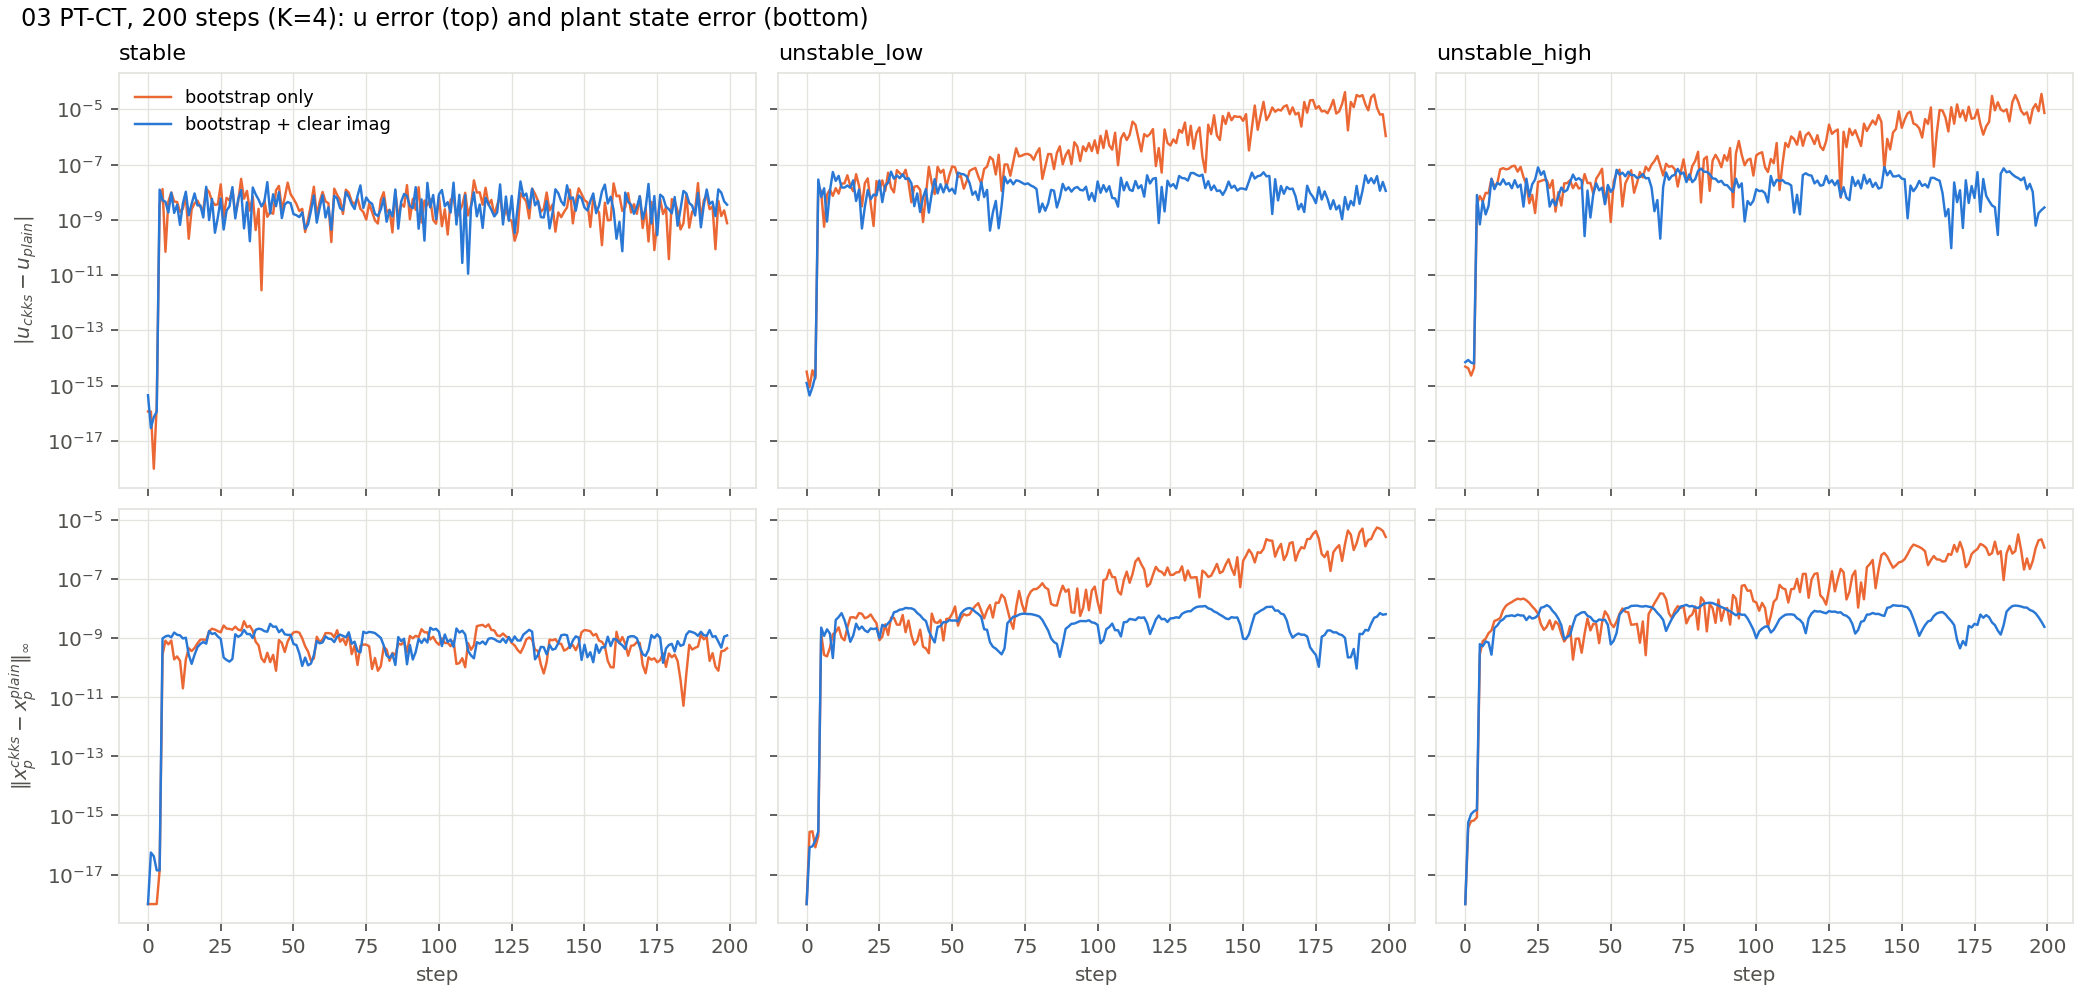
\includegraphics[width=\linewidth]{figures/clearimag_u_plant.png}
\caption{03 PT-CT, 200 step. 위: $|u_{\mathrm{ckks}}-u_{\mathrm{plain}}|$. 아래: plant 상태 오차. 주황: bootstrapping만. 파랑: bootstrapping 후 허수부 제거.}
\end{figure}
\begin{itemize}
\item 허수부를 지우면 unstable profile에서도 $u$ 오차가 $10^{-8}$ 수준에서 유지됨.
\item Plant 오차도 $2\times10^{-8}$ 이하로 유지됨.
\end{itemize}

\subsection{05 CT-CT: 지연 입력창 ARX ($N=4096$)}
\begin{itemize}
\item 조건: $N=4096$ 연구용 파라미터, 200 step, $d=K$ (따로 표시한 경우 제외), 허수부 제거.
\item $K\le16$에서는 $\rho(F^{K-1}\Fb)\le0.79<1$이라 $d=K$여도 유계임 (\S\ref{sec:dstab}).
\item 비교한 세 구현:
  \begin{itemize}
  \item \emph{스칼라}: 모든 항을 sparse scalar 곱셈으로 계산.
  \item \emph{출력 패킹}: \texttt{--pack-y}.
  \item \emph{출력+입력창 패킹}: \texttt{--pack-y --pack-u}.
  \end{itemize}
\item 최소 $T_s$는 측정 시간 기반 실시간 스케줄 모델 값임.
  \begin{itemize}
  \item 서버는 $y(t)$ 수신 즉시 $u(t)$를 계산함.
  \item 별도 작업자가 bootstrapping을 FIFO로 처리함.
  \item 실제 병렬 실행이 아님.
  \end{itemize}
\end{itemize}

\begin{table}[H]
\centering
\small
\begin{tabular}{llrrrr}
\toprule
구현 & $K$ & 최대 $u$ 오차 & bt/step & $u$ 계산 [ms] & 최소 $T_s$ [ms] \\
\midrule
스칼라 & 4 & $1.2\times10^{-12}$ & 0.96 & 46.5 & 385 \\
       & 8 & $7.4\times10^{-13}$ & 0.46 & 74.7 & 194 \\
       & 16 & $3.4\times10^{-13}$ & 0.22 & 141 & 500$^\ast$ \\
출력 패킹 & 4 & $1.1\times10^{-12}$ & 0.96 & 33.0 & 375 \\
          & 8 & $6.1\times10^{-13}$ & 0.46 & 36.4 & 191 \\
          & 16 & $8.1\times10^{-13}$ & 0.22 & 41.0 & 99 \\
출력+입력창 패킹 & 4 & $7.9\times10^{-13}$ & 0.24 & 32.3 & 106 \\
                 & 8 & $5.8\times10^{-13}$ & 0.115 & 38.5 & 62 \\
                 & 16 & $4.4\times10^{-13}$ & 0.055 & 43.0 & 62 \\
\midrule
스칼라, $d=1$ & 4 & $1.1\times10^{-12}$ & 0.98 & 34.0 & 496 \\
스칼라, 허수부 유지 & 4 & $8.5\times10^{-11}$ (증가) & 0.96 & 48.7 & 409 \\
출력+입력창 패킹, 500 step & 4 & $7.9\times10^{-13}$ & 0.25 & 33.1 & 115 \\
출력 패킹, 500 step & 16 & $6.8\times10^{-13}$ & 0.24 & 42.2 & 103 \\
\bottomrule
\end{tabular}
\caption{05 CT-CT, \texttt{unstable\_low}. 최대 $u$ 오차: $\max_t|u_{\mathrm{ckks}}-u_{\mathrm{plain}}|$. bt/step: step당 bootstrapping 횟수. $u$ 계산: 평균, register 갱신 포함. $^\ast$ 한 step의 일시적 지연(500\,ms) 때문이며 평균은 141\,ms. Bootstrapping 1회 약 370--450\,ms.}
\label{tab:05}
\end{table}

\begin{itemize}
\item 다른 profile (출력+입력창 패킹, $K=4/8/16$):
  \begin{itemize}
  \item \texttt{stable}: 최대 오차 $3\times10^{-14}$ 이하, 최소 $T_s$ 105/76/53\,ms.
  \item \texttt{unstable\_high}: 최대 오차 $1.2\times10^{-12}$ 이하, 최소 $T_s$ 122/63/59\,ms.
  \end{itemize}
\end{itemize}

\begin{figure}[H]
\centering
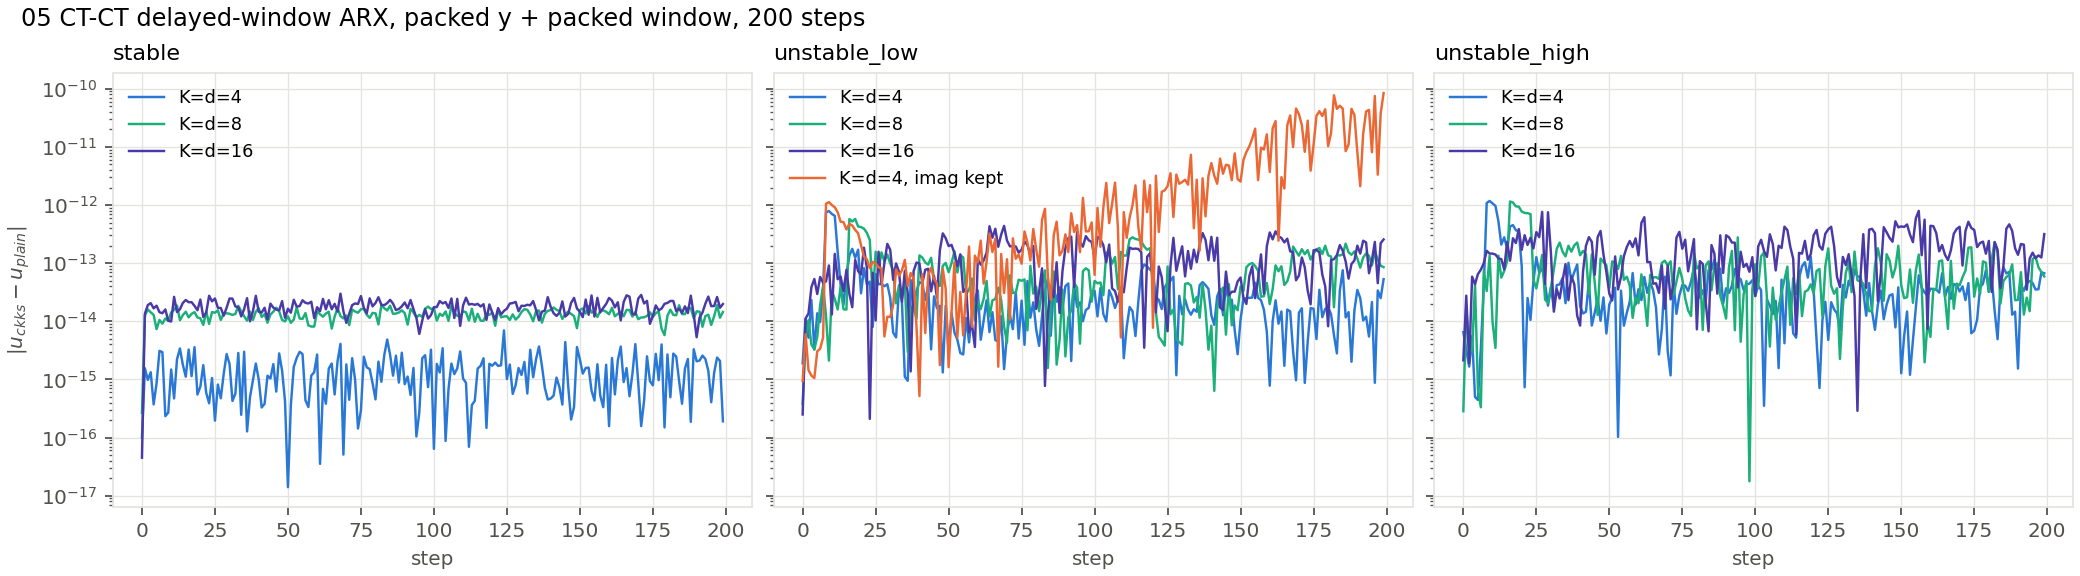
\includegraphics[width=\linewidth]{figures/arx_packyu_u_error.png}
\caption{05 CT-CT (출력+입력창 패킹), 200 step, $|u_{\mathrm{ckks}}-u_{\mathrm{plain}}|$. \texttt{unstable\_low}의 주황선은 허수부를 지우지 않은 경우 ($K=d=4$, 스칼라).}
\end{figure}

\begin{figure}[H]
\centering
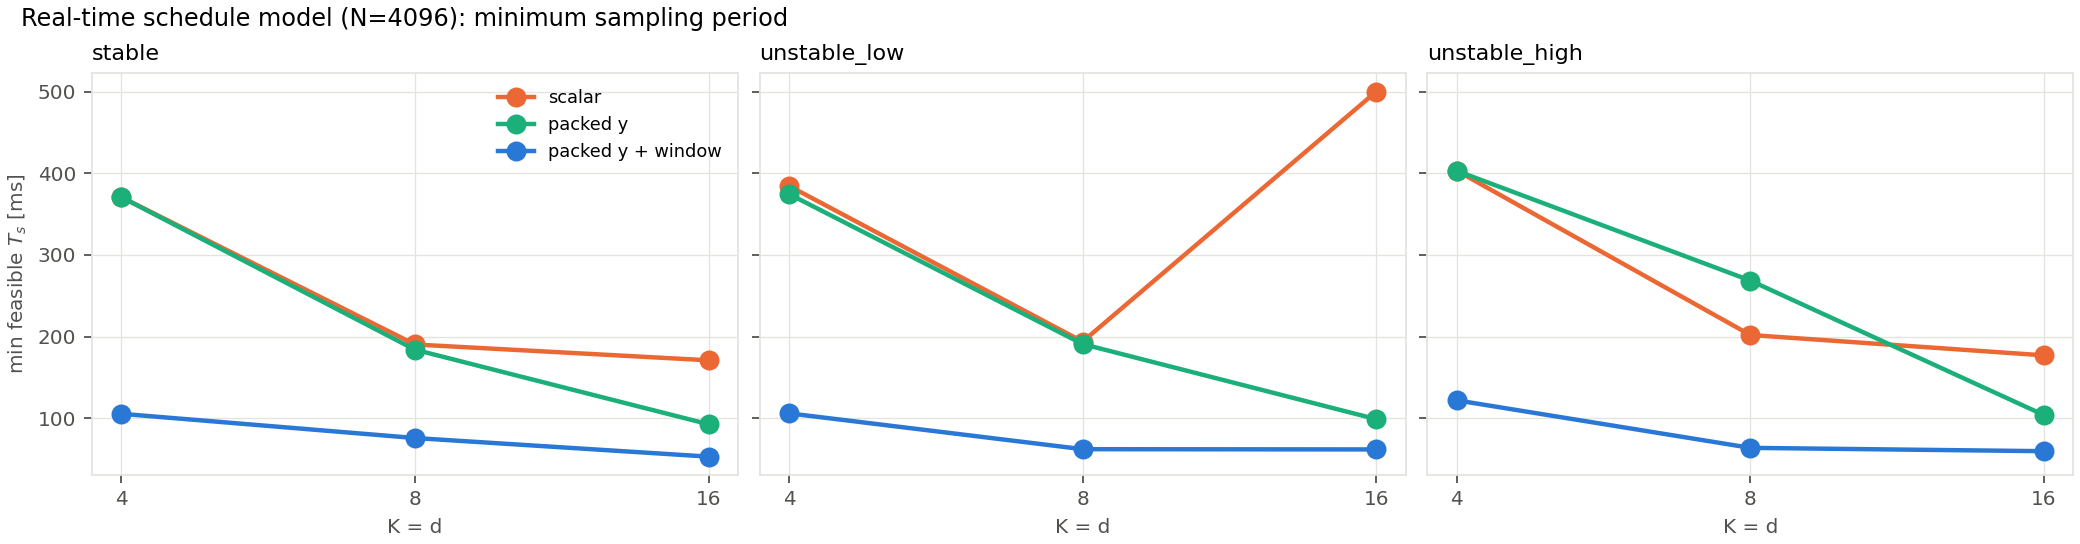
\includegraphics[width=\linewidth]{figures/arx_min_Ts.png}
\caption{실시간 스케줄 모델의 최소 sampling period ($N=4096$).}
\end{figure}

\paragraph{관찰.}
\begin{itemize}
\item \textbf{정확도와 유계성.}
  \begin{itemize}
  \item 모든 설정에서 $u$ 오차 $1.6\times10^{-12}$ 이하이고 시간에 따라 증가하지 않음.
  \item 500 step도 200 step과 같은 수준임. Register와 창 단위 bootstrapping에서 노이즈가 누적되지 않음.
  \item \texttt{unstable\_high}도 같은 수준임.
  \end{itemize}
\item \textbf{계수 증가.}
  \begin{itemize}
  \item 계수는 $\rho(F)^{2K-2}$로 커짐 ($K=16$에서 $\max|\alpha|\approx2.5$).
  \item $K=16$까지는 오차가 커지지 않음. Bootstrapping 횟수 감소 효과가 더 큼.
  \end{itemize}
\item \textbf{허수부.}
  \begin{itemize}
  \item 지우지 않으면 CT-CT ARX에서도 오차가 약 $2\times10^{-13}$에서 $10^{-11}$ 이상으로 증가함.
  \item 허수부 오차 추정치도 10\,bit에서 26\,bit로 증가함. 지우면 7--10\,bit로 일정함.
  \end{itemize}
\item \textbf{$K$의 trade-off.}
  \begin{itemize}
  \item 스칼라 방식은 $K$에 비례해 곱셈이 늘어 $u$ 계산이 병목이 됨.
  \item 출력 패킹 후에는 $u$ 계산이 $K$에 거의 무관함 (33$\to$41\,ms).
  \item 곱셈은 5회로 고정되고, rotation만 $\log_2S$로 늘어남.
  \end{itemize}
\item \textbf{입력창 패킹.}
  \begin{itemize}
  \item Bootstrapping 횟수가 1/4로 줄어 $K=4$에서도 최소 $T_s$가 385\,ms에서 106\,ms로 줄어듦.
  \item $K\ge8$에서는 최소 $T_s$ (약 60\,ms)를 서버의 step당 계산 최댓값이 정함.
  \item 이 최댓값은 초기 구간에서 나옴 (초기 register와 다음 블록 register를 함께 갱신하는 step).
  \end{itemize}
\item \textbf{지연 $d$.}
  \begin{itemize}
  \item 같은 $K=4$에서 $d=1$은 최소 $T_s$ 496\,ms로, $d=K$ (385\,ms)보다 큼.
  \item 마지막 입력의 bootstrapping이 한 period 안에 끝나야 하기 때문임.
  \end{itemize}
\end{itemize}

\subsection{128-bit: $K$ 선택과 최종 설정}\label{sec:128}
\begin{itemize}
\item 옵션: \texttt{--secure128 --compact-inputs --pack-y --pack-u} ($N=65536$, depth 19).
\item Bootstrapping 1회 약 5--7\,s (2회 iterative + 허수부 제거 + 창 패킹 포함).
\item $u$ 계산 step당 약 150--200\,ms.
\item 따라서 \eqref{eq:Kmin}에 의해 다음이 필요함.
\end{itemize}
\begin{equation}
K\gtrsim\frac{T_{\mathrm{bt}}}{T_u}\approx34 .
\end{equation}
\begin{itemize}
\item Bootstrapping 정밀도는 $N=4096$보다 낮음 (단일 bootstrapping 약 16 bit).
\end{itemize}

\begin{table}[H]
\centering
\resizebox{\linewidth}{!}{%
\begin{tabular}{lrrrrrrr}
\toprule
설정 & step & 최대 $u$ 오차 & $\max|\alpha|$ & $T_{\mathrm{bt}}$ [s] & $u$ 계산 [ms] & 최소 $T_s$ [ms] & 메모리 [GB] \\
\midrule
\texttt{unstable\_low}, $K=d=16$ & 128 & $9.2\times10^{-8}$ & 2.5 & 5.2 & 157 & 345 & 3.1 \\
\texttt{unstable\_low}, $K=d=32$ & 192 & $8.3\times10^{-8}$ & 10.5 & 5.5 & 176 & 202 & 3.2 \\
\texttt{unstable\_low}, $K=d=64$ & 320 & $5.7\times10^{-7}$ & 187 & 5.7 & 184 & 263 & 3.6 \\
\texttt{unstable\_high}, $K=d=64$ & 1000 & \textbf{발산} (block당 6.8배) & 187 & 6.1 & -- & 261 & 3.7 \\
\midrule
\texttt{unstable\_high}, $K=64$, $d=61$ & 640 & $1.1\times10^{-7}$ & 187 & 6.1 & 191 & 307 & 3.7 \\
\texttt{unstable\_low}, $K=64$, $d=61$ & 640 & $3.3\times10^{-8}$ & 187 & 6.7 & 203 & 303 & 3.8 \\
\bottomrule
\end{tabular}}
\caption{128-bit 결과. $u$ 계산: 창 구간 평균. 최소 $T_s$: 스케줄 모델 값이며, $u$ 계산이 가끔 튀는 step의 영향을 받음.}
\label{tab:128}
\end{table}

\begin{figure}[H]
\centering
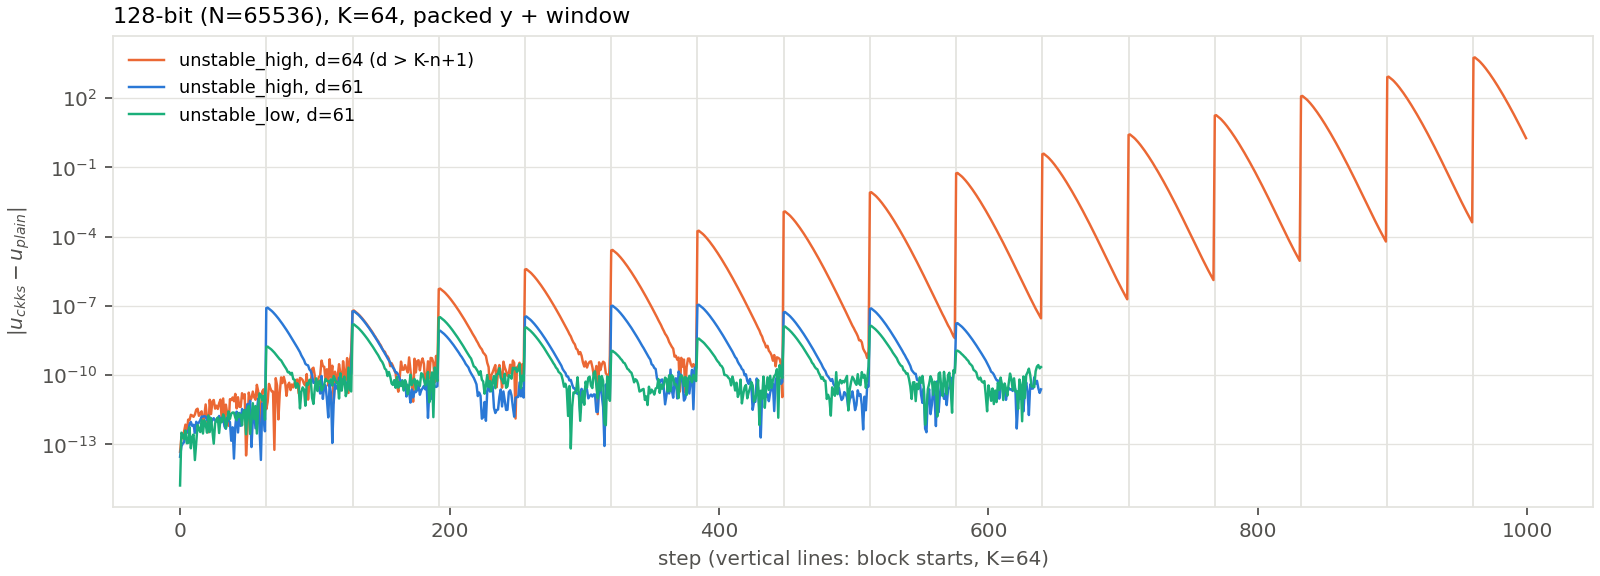
\includegraphics[width=\linewidth]{figures/final_d_stability.png}
\caption{128-bit, $K=64$. 세로선은 블록 시작. $d=64$ (주황): 블록마다 리셋 점프가 6.8배씩 커짐. $d=61$ (파랑, 초록): 점프가 약 $10^{-7}$로 일정하고 블록 안에서 폐루프로 감쇠함.}
\label{fig:final-d}
\end{figure}

\paragraph{$K$와 $d$의 선택.}
\begin{itemize}
\item \textbf{$K$의 하한 (시간).}
  \begin{itemize}
  \item $K\gtrsim T_{\mathrm{bt}}/T_u$이면 bootstrapping이 병목에서 빠짐.
  \item $K=16$: bootstrapping이 최소 $T_s$를 정함 (345\,ms $\approx T_{\mathrm{bt}}/16$).
  \item $K\ge32$: $u$ 계산이 정함.
  \end{itemize}
\item \textbf{$K$의 대가 (정확도).}
  \begin{itemize}
  \item 계수가 $\rho(F)^{2K-2}$로 커짐 ($K=64$: $\max|\alpha|=187$, $\max|\beta|=319$).
  \item Bootstrapping 오차가 증폭되어 128-bit $K=64$의 오차는 $10^{-7}$ 수준임.
  \item 발산하지 않는 한 이 정도는 허용 범위로 봄.
  \end{itemize}
\item \textbf{$d$ (안정성).}
  \begin{itemize}
  \item $d\le K-n+1$이어야 리셋 점프가 누적되지 않음.
  \item $d=K-n+1$이면 여유는 $K-n+1$ period임.
  \end{itemize}
\item \textbf{최종 설정: $K=64$, $d=61$.}
  \begin{itemize}
  \item Bootstrapping 여유는 다음과 같음. $T_{\mathrm{bt}}\approx6$\,s의 약 3배임.
  \end{itemize}
\end{itemize}
\begin{equation}
d\,T_s\approx61\times0.3\,\mathrm{s}\approx18\,\mathrm{s}.
\end{equation}
\begin{itemize}
\item[]
  \begin{itemize}
  \item $K=32$도 시간 조건은 만족하지만 여유가 약 1.2배뿐임. Bootstrapping 시간 변동(5--7\,s)에 취약함.
  \end{itemize}
\end{itemize}

%==========================================================================
\section{남은 과제}
\begin{itemize}
\item 실제 병렬 실행(bootstrapping 작업자 분리)으로 스케줄 모델을 검증함.
      현재 최소 $T_s$는 bootstrapping과 $u$ 계산이 다른 자원에서 돈다는 가정의 값임.
\item 128-bit 최종 설정을 더 긴 시간(수천 step)으로 확인함.
\item 초기 구간과 register 갱신이 겹치는 step의 계산 최댓값을 줄여 최소 $T_s$를 낮춤.
\item 복호화 noise flooding 모드와 허수부 제거의 상호작용을 정리함.
\item 04 CT-CT와 동일 조건에서 장기(수천 step) 실행으로 비교함.
\item 4-tank 등 물리 plant 모델로 확장함.
\end{itemize}

\begin{thebibliography}{9}
\bibitem{kim} J.~Kim, ``Further methods for encrypted linear dynamic controllers utilizing re-encryption,'' arXiv:2307.16445, 2023.
\bibitem{openfhe-nf} OpenFHE, ``CKKS noise flooding,'' \texttt{src/pke/examples/CKKS\_NOISE\_FLOODING.md}, v1.5.1.
\bibitem{kimsong} D.~Kim and Y.~Song, ``Approximate homomorphic encryption over the conjugate-invariant ring,'' ICISC 2018 (LNCS 11396, 2019).
\end{thebibliography}
\end{document}
